\documentclass{article}
\usepackage{babel}
\usepackage{graphicx}
\usepackage[hidelinks]{hyperref}
\usepackage{tabularx}
\usepackage[paper=portrait,pagesize]{typearea}

\graphicspath{{images/}}

\title{
\includegraphics[width=10cm]{logo/logo_cz.png}\\Formálne jazyky a prekladače \\ 
Dokumentácia k prekladaču jazyka IFJ26}
\author{\textbf{Jakub Dufek}, Samuel Vít Lehotský, Šimon Greger, Ondrej Kycl \\ \textbf{274855}, xlehots00, xgreges00, xkyclon00}
\date{\today}    

\begin{document}
    \maketitle

    \vspace{1.5em}
    {\large
    \noindent\textbf{Zovlená varianta:}

    \hspace*{0.25cm}Výškovo vyvážený binárny vyhľadávací strom (vv-BVS)\vspace{1.5em}

    \noindent\textbf{Rozdelenie bodov:}

    \begin{tabular}{ll}
      274855:    &  100\\
      xlehots00: &  100\\
      xgreges00: &  100\\
      xkyclon00: &  100\\
    \end{tabular}\vspace{1.5em}

    \noindent\textbf{Implementované rozšírenia:}
    
    \begin{tabular}{l}
      BOOLTHEN\\
    \end{tabular}\vspace{1.5em}

    \noindent\textbf{GitHub repozitár:}
    
    \hspace*{0.25cm}\href{https://github.com/Jakub-Dufek/IFJ-project-2026-compiler.git}{IFJ-project-2026-compiler.git}
    } 

    \newpage

    \tableofcontents

    \newpage

    \section{Úvod}

\vspace{1.5em}
{ \large 

\noindent\textbf{Rozdelenie práce:}
\vspace{0.75em}

\noindent Práca aj bodové ohodnotenie boli medzi členov tímu rozdelené rovnomerne.

\vspace{0.75em}
\noindent
\begin{tabularx}{\textwidth}{@{} l @{\hspace{1.5em}} >{\raggedright\arraybackslash}X @{}}
  x274855:    &  Syntaktický analyzátor, dynamická pamäť prekladača, spracovanie chýb\\
  xlehots00: &  Lexikálny analyzátor, Analyzátor výrazov, generovanie vstavaných funkcií, dokumentácia\\
  xgreges00: &  Lexikálny analyzátor, Generátor cieľového kódu\\
  xkyclon00: &  Sémantický analýzátor, Tabuľka symbolov\\
\end{tabularx}

\vspace{1.5em}

\noindent\textbf{Popis práce v týme:}

\vspace{0.75em}
\noindent Každý týždeň v nedeľu o 19:00 hodine sa konalo stretnutie členov týmu. Na tomto stretnutí sme si prešli prácou spravenou cez týždeň, ktorá bola prebraná a schválená, následne sa prebralo, čo je ešte potrebné spraviť, prípadne čo má najvyšiu prioritu a rozdelila sa práca na ďalší týždeň.

\vspace{0.75em}
\noindent Schvaľovanie zmien v repozitár: Každá časť prekladača bola vyvíjaná vo vlastnej vetve, pričom pri komplexnejších moduloch sme vytvárali vetvy iteratívne (označené \verb|1.0|, \verb|2.0|, \verb|3.0|). Zmeny sa do vetvy ukladali až potom, čo bolo možné projekt lokálne preložiť. Priebežný vývoj bol ukladaný do vetvy \verb|semnatic-analysis| (neskôr \verb|semantic-analysis-2|), ktorá bola do hlavnej vetvy \verb|main| zlučovaná na nedeľných stretnutiach až po dokončení ucelenej časti projektu, jej schválenáním členmi tímu ako aj úspešním vykonaním všetkých testov.

\vspace{0.75em}
\noindent Testovali sme prostredníctvom troch pripravených testovacích programov (\verb|tiny_prog.scala|, \verb|small_prog.scala|, \verb|medium_prog.scala|), z ktorých každy rozširoval ako dĺžku programu, tak aj komplexnosť príkazov na preloženie prekladačom.
\newpage
\vspace{0.75em}
\noindent Kód sme uniformne formátovali prostredníctvom \verb|.clang-format|, ktorý sme nastavili nasledovne:\\

\vspace{0.75em}
\noindent
\begin{tabular}{l l}
  Odsadenie riadka: & 4 znaky\\
  Maximálna dĺžka riadka: & 130 znakov\\
  Umiestnenie znaku ukazateľa (\verb|*|) a referencie (\verb|&|): & vpravo \\
  Konvencia umiestnenia označenia rozsahu kódu: & Stroustrup \\
  Maximálny počet prázdnych riadkov: & 3
\end{tabular}
\hspace*{0.25cm}
}\newpage
    \KOMAoptions{paper=landscape,pagesize}
    \section{Blokové schéma architektúry}

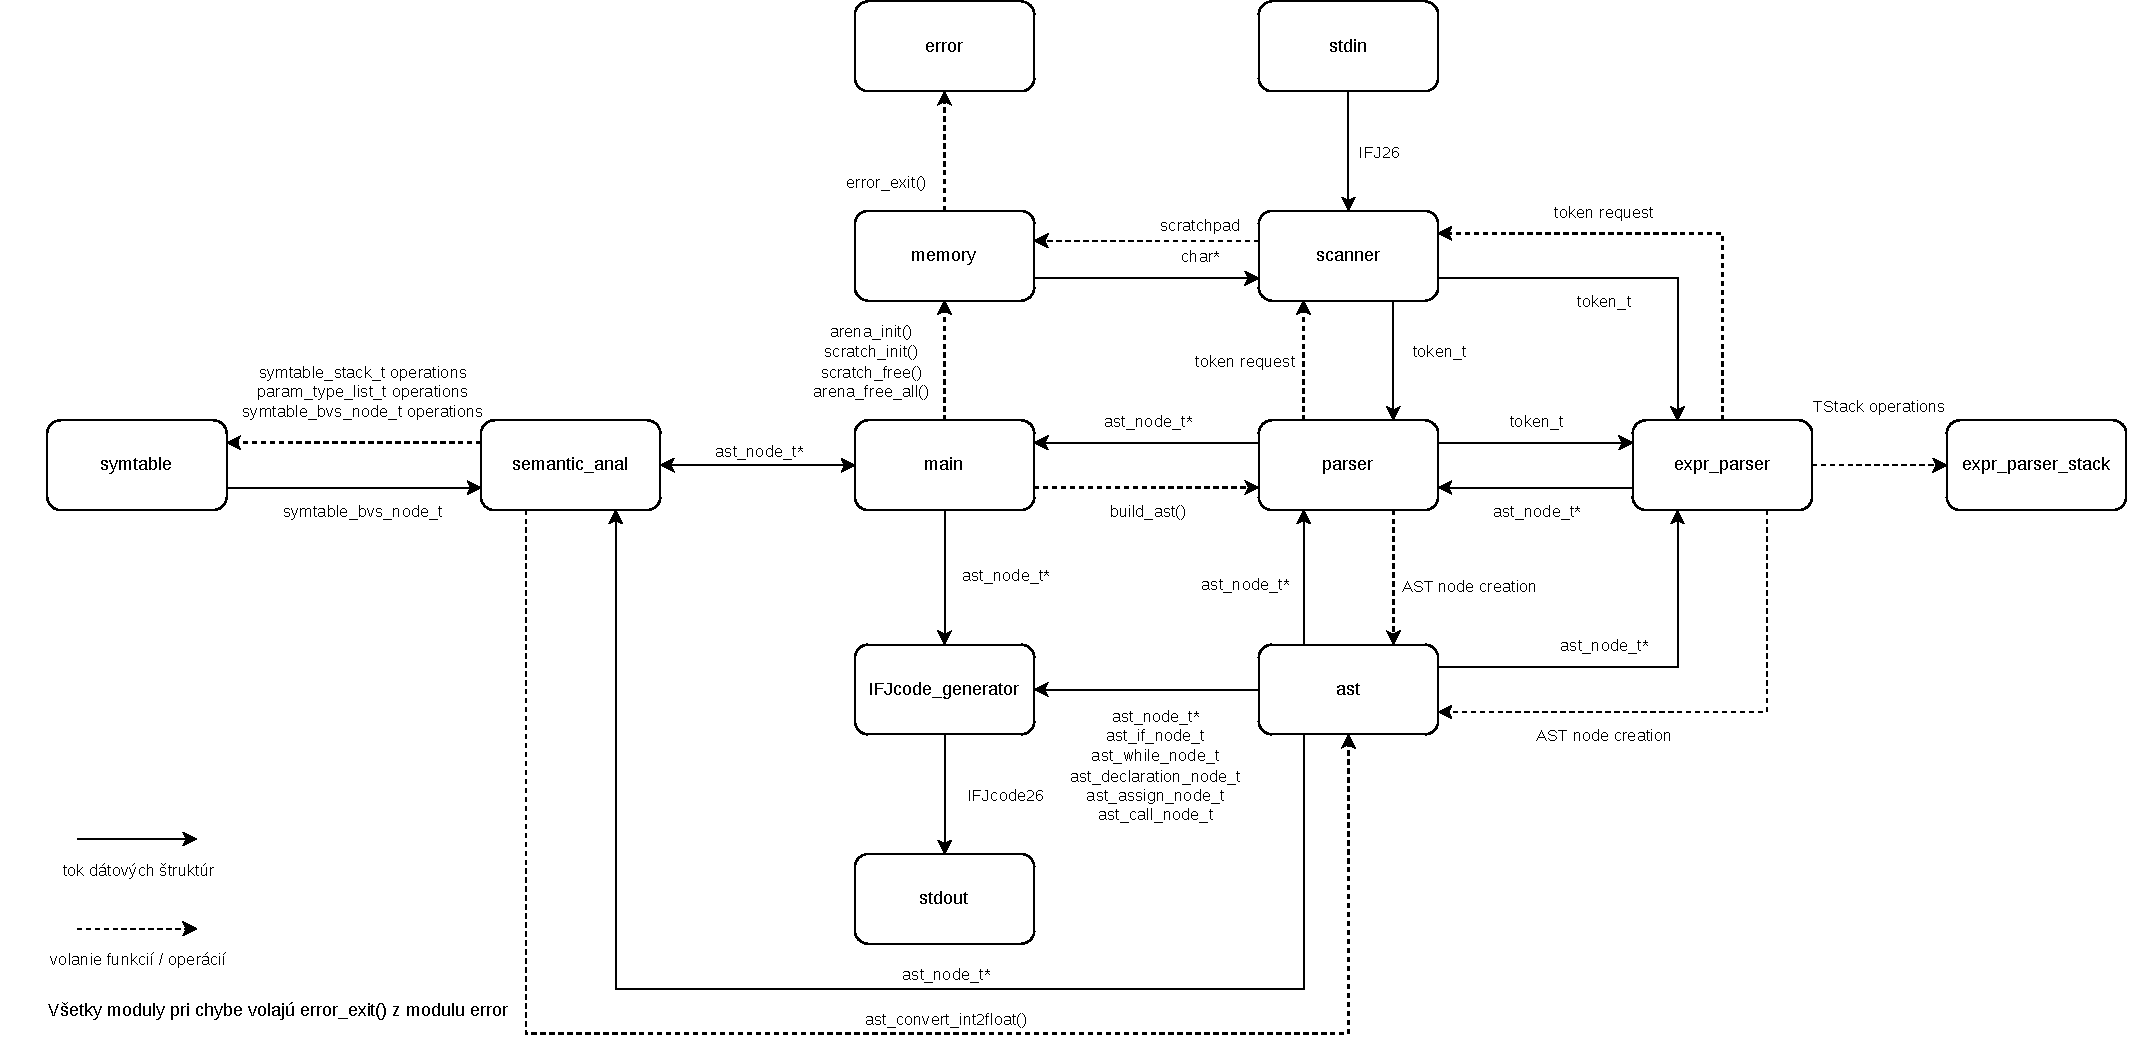
\includegraphics[width=1.8\linewidth]{img/IFJ.drawio.pdf}\newpage
    \section{Diagram automatu lexikálneho analyzátora}\newpage
    \KOMAoptions{paper=portrait,pagesize}
    \section{Moduly}

\vspace{1.5em}
{ \large \raggedright
\begin{itemize}
    \item \verb|scanner.c / scanner.h|
    \begin{itemize}
        \item Modul, reprezentující lexikální analyzátor implementovaný pomocí konečného automatu. Modul se používá zavoláním jeho vstupní funkce \verb|get_token()|, která přečte jeden lexém ze vstupu, vytvoří z něj token a tento token vrátí.
    \end{itemize}
    \item \verb|parser.c /parser.h|
    \begin{itemize}
        \item Modul, reprezenující syntaktický analyzátor implementovaný pomocí metody rekurzivního sestupu. Modul se používá zavoláním jeho funkce \verb|build_ast()|, která spustí smyčku analýzy. Vrátí vybudovaný strom.
    \end{itemize}
    \item \verb|ast.c / ast.h|
    \begin{itemize}
        \item Pomocný modul k modulu \verb|parser.c| a \verb|expr_parser.c| alokující jednotlivé uzly AST.
    \end{itemize}
    \item \verb|expr_parser.c / expr_parser.h| 
    \begin{itemize}
        \item Modul, ktorý využíva syntaktická analýza na spracovávanie výrazov a tvorbu ich abstraktného syntaktického stromu (AST). Základom modulu je precedenčná tabuľka, na základe ktorej sa volí operácia spracovania, a to podľa najvyššieho terminálu na zásobníku a nasledujúceho vstupného tokenu.
    \end{itemize}
    \item \verb|expr_parser_stack.c / expr_parser_stack.h|
    \begin{itemize}
        \item Pomocný modul k modulu \verb|expr_parser|, obsahujúci funkcie implementujúce zásobník \verb|TStack|, využívaný na uchovávanie tokenov a (ne)terminálov práve spracovávaného výrazu.
        \item Implementácia základných operácií (\verb|stack_push|, \verb|stack_pop|, \verb|top|, \verb|empty|) zásobníka, vychádzá z algoritmov uvedených v 3. prednáške predmetu IAL [1, slajdy 14-16] a je doplnená o pomocné operácie \verb|top_terminal| a \verb|stack_push_after_top_terminal|.
    \end{itemize}
    \newpage
    \item \verb|memory.c / memory.h|
    \begin{itemize}
        \item Pomocný modul, implementující struktury Arena a Scratchpad. Arena slouží pro data potřebná po celou dobu běhu programu, tj. uzly AST a řetězce identifikátorů.
        \item Značná část tohoto modulu byla implementovaná pomocí AI, konkrétně modelu Gemini Flash 3.8.
    \end{itemize}
    \item \verb|semantic_anal.c / semantic_anal.h|
    \begin{itemize}
        \item Tento modul provádí sémantickou analýzu, tedy kontroluje a obohacuje výstup syntaktické analýzy za využití tabulky symbolů.
    \end{itemize}
    \item \verb|symtable.c / symtable.h|
    \begin{itemize}
        \item Tento modul obsahuje implementaci tabulky symbolů pomocí AVL stromu, seznamu typů parametrů, a zásobníku tabulek symbolů. 
        \item Implementácia štruktúry zásobníka (\verb|symtable_stack_t|) a jeho základných operácií (\verb|symtable_stack_initialize|, \verb|symtable_stack_push|, \verb|symtable_stack_pop|, \verb|symtable_stack_is_empty|) vychádzá z algoritmov uvedených v 3. prednáške predmetu IAL [1, slajdy 14-16]
        \item Implementácia Výškovo vyváženého binárního vyhledávacího stromu (\verb|bvs_max|, \verb|bvs_height|) vychádzá z algoritmov uvedených v 4. prednáške predmetu IAL [2, slajd 27]
        \item Implementácia Výškovo vyváženého binárního vyhledávacího stromu (\verb|symtable_find_symbol|, \verb|symtable_create_node|, \verb|symtable_insert|, \verb|symtable_right_rotate|, \verb|symtable_left_rotate|) vychádzá z algoritmov uvedených v 5. prednáške predmetu IAL [3, slajdy 18, 22, 23, 51]
    \end{itemize}
    \item \verb|IFJcode_generator.c / IFJcode_generator.h|
    \begin{itemize}
        \item Modul, který rekurzivně zpracovává obsah abstraktního syntaktického stromu, na jehož základě na standardní výstup vypisuje jeho interpretaci pomocí jazyka IFJcode26.
    \end{itemize}
    \newpage
    \item \verb|error.c / error.h|
    \begin{itemize}
        \item Pomocný modul, který uvolňuje alokovanou paměť v případě chyby překladače, vypíše chybu na chybový výstup a skončí s příslušným error kódem.
    \end{itemize}
    \item \verb|structures.h|
    \begin{itemize}
        \item Knihovna obsahující definici struktury \verb|token_t| a hodnot specifické pro token. Struktura \verb|token_t| slouží jako reprezentace jednoho tokenu, který vyrábí scanner a využívá parser.
    \end{itemize}
\end{itemize}

%Generated from code in expr_parser.c by Google Gemini 4 Neon
%Promt: Prepíš mi túto tabuľku do LaTeXu (bez komentárov)
\newpage
\noindent\textbf{Precedenčná tabuľka:}\\
\vspace{0.75em}
\begin{tabular}{|c|c|c|c|c|c|c|c|c|c|c|c|}
\hline
 & \texttt{+-} & \texttt{*/} & \texttt{\&\&} & \texttt{||} & \texttt{<><=>=} & \texttt{==!=} & \texttt{(} & \texttt{)} & \texttt{-i!i} & \texttt{i} & \texttt{\$} \\ \hline
\texttt{+-}     & $>$ & $<$ & $>$ & $>$ & $>$ & $>$ & $<$ & $>$ & $<$ & $<$ & $>$ \\ \hline
\texttt{*/}     & $>$ & $>$ & $>$ & $>$ & $>$ & $>$ & $<$ & $>$ & $<$ & $<$ & $>$ \\ \hline
\texttt{\&\&}   & $<$ & $<$ & $>$ & $>$ & $<$ & $<$ & $<$ & $>$ & $<$ & $<$ & $>$ \\ \hline
\texttt{||}     & $<$ & $<$ & $<$ & $>$ & $<$ & $<$ & $<$ & $>$ & $<$ & $<$ & $>$ \\ \hline
\texttt{<><=>=} & $<$ & $<$ & $>$ & $>$ &     & $>$ & $<$ & $>$ & $<$ & $<$ & $>$ \\ \hline
\texttt{==!=}   & $<$ & $<$ & $>$ & $>$ & $<$ &     & $<$ & $>$ & $<$ & $<$ & $>$ \\ \hline
\texttt{(}      & $<$ & $<$ & $<$ & $<$ & $<$ & $<$ & $<$ & $=$ & $<$ & $<$ &     \\ \hline
\texttt{)}      & $>$ & $>$ & $>$ & $>$ & $>$ & $>$ &     & $>$ &     &     & $>$ \\ \hline
\texttt{-i!i}   & $>$ & $>$ & $>$ & $>$ & $>$ & $>$ & $<$ & $>$ & $<$ & $<$ & $>$ \\ \hline
\texttt{i}      & $>$ & $>$ & $>$ & $>$ & $>$ & $>$ &     & $>$ &     &     & $>$ \\ \hline
\texttt{\$}     & $<$ & $<$ & $<$ & $<$ & $<$ & $<$ & $<$ &     & $<$ & $<$ &     \\ \hline
\end{tabular}
}\newpage
    \section{Zdroje a AI}

\vspace{1.5em}
{ \large \sloppy
\noindent\textbf{Zdroje:}

\vspace{0.75em}
\noindent [1] IAL - Algoritmy: 3. prednáška (Abstraktné dátové typy II.) Brno: Fakulta informačních technológií VUT v Brně, 2026 [cit. 2026-11-21]

\vspace{0.75em}
\noindent [2] IAL - Algoritmy: 4. prednáška (Stromové dátové štruktúry) Brno: Fakulta informačních technológií VUT v Brně, 2026 [cit. 2026-11-21]

\vspace{0.75em}
\noindent [3] IAL - Algoritmy: 6. prednáška (Vyhľadávacie tabulky II.) Brno: Fakulta informačních technológií VUT v Brně, 2026 [cit. 2026-11-21]

\vspace{0.75em}
\noindent Všetky materiály sú dostupné z e-learningového portálu VUT v Brně (Moodle), kurz Algoritmy (IAL 26/27Z)

\vspace{1.5em}

\noindent\textbf{Využitie AI:}

\vspace{0.75em}
\noindent Nástroje AI sme využívali v súlade zo zadaním. Primárne na objasnenie zadania a pri hladaní problémov a chýb.

\vspace{0.75em}
\noindent Príklad: Ahoj mám v AST navrženou strukturu pro deklaraci proměnné a teď vytvářím definici funkce, napadlo mě, že [...]. Je to správný přístup? Negeneruj kód, pouze diskutuj a klaď řečnické otázky které prohloubí mé přemýšlení o formálních jazycích. 
}\newpage
    
\end{document}
